\documentclass[12pt]{article}
\usepackage[utf8]{inputenc}
\usepackage{geometry}
\usepackage{pdfpages}
\geometry{a4paper, top=1.25cm,bottom=1.5cm,right=1.5cm,left=1.5cm}
\usepackage{amsmath, amssymb, amstext}
\usepackage{tikz}
\setlength\parindent{0pt}
\tikzset{myBound/.style={color=blue}}
\tikzset{myAxisLine/.style={line width=0.3mm,color=black}}
\tikzset{myLine/.style={thick,color=black}}
\usepackage{enumitem}
\usepackage{array}
\newcolumntype{M}{> {$} l < {$}}
\usepackage{mathtools}
\newcommand\Mycomb[2]{\prescript{#1\mkern-1mu}{}C_{#2 \mkern+6mu}}
\renewcommand{\baselinestretch}{1.2}
\usepackage{tkz-euclide}
\usetikzlibrary{positioning}

\usepackage{hyperref}
\hypersetup{
	colorlinks=true,
	linkcolor=blue,
	filecolor=magenta,      
	urlcolor=cyan,
}

\definecolor{minGridCol}{RGB}{130, 255, 255}
\definecolor{gridCol}{RGB}{0,230,230}
\tikzset{myMajGrid/.style={color=gridCol, line width=0.0mm}}
\tikzset{myMinGrid/.style={color=minGridCol, line width=0mm}}
\tikzset{myAxisLine/.style={line width=0.3mm,color=black}}
\tikzset{myTick/.style={color=black, line width=0.3mm}}

\usepackage{tkz-euclide}

\tikzset{myAngle/.style={thin,color=black}}
\newcommand\onelabel[6]{
	\tkzMarkAngle[myAngle,size =#1]({#2},{#3},{#4})
	\tkzLabelAngle[pos=#5 ]({#2},{#3},{#4}){\footnotesize ${#6}$}
}

\title{Sequences and Series}
\author{Kh notes}
\date{}



%----------------------Triangles------------------------------------------
\newcommand{\x}{0}
\newcommand{\y}{0}
\newcommand\triangleSAS[7]{
	\renewcommand{\x}{0};
	\renewcommand{\y}{0};
	\coordinate (R) at (#5,#6);
	%\filldraw[red](\x,\y) circle [radius=1pt];
	%\filldraw[](0,0) circle[radius=1pt];
	\begin{scope}[ xshift=#5cm, yshift=#6cm,rotate around={#4:(R)}, scale around={#7:(R)} ]
		%\filldraw[blue](\x,\y) circle [radius=1pt];
		\coordinate(O) at(0,0);
		\coordinate(B) at (#3,0);
		\coordinate(A) at ({#1*cos(#2)},{#1*sin(#2)});		
	\end{scope}
	
}


%----------------------Bounding Boxes------------------------------------------
\newcommand\brect[2]{
	\draw[myBound](-#1,-#2)rectangle(#1,#2);
	%backcolour
	\draw[myBound, opacity=0.1, xstep=0.5cm, ystep=0.5cm](-#1,-#2)grid(#1,#2);
	\draw[myBound](0,0)circle[radius=2pt];
}
\begin{document}
	\maketitle
\tableofcontents
\newpage
\section{Introduction (Number Sequences)}
\begin{center}
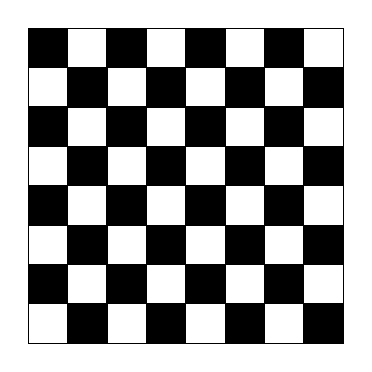
\begin{tikzpicture}
	\draw[](0,0)rectangle(4,4);
	\draw[xstep=0.5, ystep=0.5](0,0)grid(4,4);
	\newcommand{\shft}{0.5}
	\foreach \r in {0,1,2,3}{
		\foreach \c in {0,1,2,3}{
		\fill[](\c,\r +\shft)rectangle(\c +\shft,\r +2*\shft);
	}
	
	}
		\foreach \r in {0,1,2,3}{
		\foreach \c in {0,1,2,3}{
			\fill[](\c +\shft,\r )rectangle(\c +2*\shft,\r +\shft);
		}
	}
\end{tikzpicture}
\end{center}
Grains of rice problem.\\
How do we define this problem mathematically?
\begin{itemize}
	\item Create a number sequence for each square: $1,2,4,8,16,..., 2^{62},  2^{63}$
	\item Consider relations between the number in each square: $s_2 = 2s_1$, or $s_9= 2^8$
	\item Create a formula for each square: $s_n = 2^{n-1}$
	\item Communicate the idea of summing : $\displaystyle 1+2+4+8+16,+...+, 2^{62}+2^{63} = \sum_{i=1}^{64} 2^{i-1}$
	\item Actually solve the problem  $1+2+4+8+16,+...+, 2^{62}+2^{63} = ?$
\end{itemize}
Consider:
\begin{align*}
	1+1+2+4+8 = 2+2+4+8\\
	=2(1+1+2+4)\\
		=2(2+2+4)\\
		=2(2(1+1+2))\\
		=2(2(2+2))\\
		=2(2(2(1+1)))\\
		=2(2(2(2)))
		=2^4
\end{align*}
\newpage
\section{Arithmetic Sequences}
An example of an arithmetic sequence is:
\LARGE $$14,17, 20, 23,...$$ \normalsize
An arithmetic sequence has a common difference between the terms (in this case 3)
\begin{itemize}
	\item We need to be able to descibe the sequence:\\
	\textbf{The sequence has a first term of 14 and increases by 3 each time}
	\item We define $u_n$ to be the $n^{th}$ term of the sequence
	\item Unless otherwise stated $u_1$ is the first term.
	\item We define $d$ as the common difference ($d=u_{n+1} - u_{n}$).
	\item $\{u_n\}$ represents the whole sequence.
\end{itemize}
Note: the sequence is linear (so the difference is the gradient).

\begin{center}
	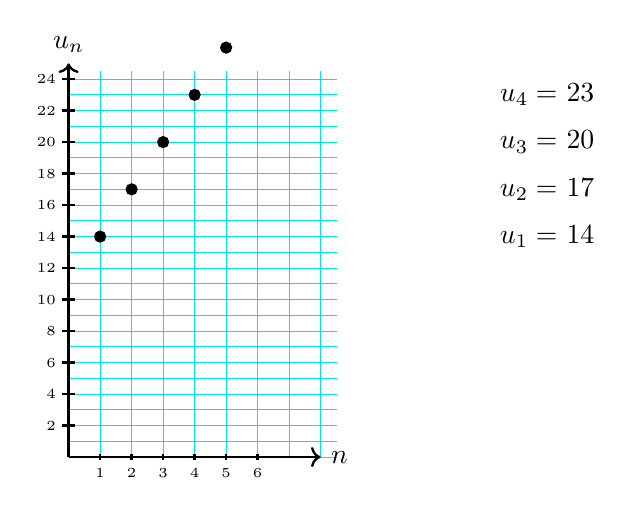
\begin{tikzpicture}[xscale=0.4, yscale=0.2]

	\draw[myMajGrid](0,0) grid(8.5,24.5);
	\draw[myAxisLine, ->](0,0)--(8,0)node[right]{$n$};
	\draw[myAxisLine, ->](0,0)--(0,25)node[above]{$u_n$};
	\foreach \n [count=\i] in{1,2,...,6 }{
		\draw[](\n,-0.1)node[below]{\tiny \n};
		\draw[myTick](\n,0.2)--(\n,-0.2);
	
	}
		\foreach \n [count=\i] in{2,4,6,...,24 }{

		\draw[](-0.1,\n)node[left]{\tiny \n};
		\draw[myTick](0.2,\n)--(-0.2,\n);
	}
	\foreach \n in{1,2,...,5}{
		\filldraw[yscale=2](\n,{(3*\n+11)/2} ) circle[radius=5pt];
	}

	\newcommand{\calc}{0};
	\foreach \x/\y in {1/0,2/0,3/0,4/0}{
		\renewcommand{\calc}{3*\x+11};	
		\draw[](17,\calc)node[left]{ $u_{\x}=$ \fpeval{\calc} };
		%\draw[<-, dashed](12,\calc)--(14,\calc);
	}	
\end{tikzpicture}
\end{center}
The middle of any three consectutive terms is the arithmetic mean of the other two terms.\\
\hrule\vspace{0.5cm}
General term formula:
\LARGE $$u_n = u_1 + (n-1)d$$\normalsize
\hspace{1cm}(this can then be simplified to a `$y=mx+c$' form)

\vspace{0.5cm}\hrule

	
\subsection{Ex 5B.1}
\begin{itemize}
	\item Showing and proving a sequence is arithmetic, 
	\item Finding terms 
	\item Working with $k$
	\item Inserting terms between
\end{itemize}
%\includegraphics[page=1,scale=0.75]{ArithmeticQuestions.pdf} 
\includepdf[pages={1-},scale=0.85]{ArithmeticQuestions.pdf} 
\subsection{Ex 5B.2}
\begin{itemize}
	\item Approximations using arithmetic sequences
\end{itemize}
\section{Geometric  Sequences}
\subsection{Ex 5C}
\section{Growth and Decay}
Starter Questions:
\begin{enumerate}
	\item A school had 1200 students and a year later this has increased by 8\% . How many students are now in the school?
	\item Mary buys a car for \$40,000 and in one year its price has decreased by 12\%. What is the value of it now?
	\item The population of Sydney is currently 5.2 million. If it increases at a rate of 1.25\% annually, what will the population be after 3 years?
\end{enumerate}
\subsection{Ex 5D}
\section{Financial Mathematics}
\subsection{Compound Interest}
\hrule\vspace{0.5cm}

\LARGE $$u_n = u_0(1+i)^n$$ \normalsize

\hspace{1cm}$u_0$ Initial Investment (Principal)

\hspace{1cm}$i$ Interest rate per compounding period

\hspace{1cm}$n$ Number of periods

\hspace{1cm}$u_n$ The final value of the investment

\vspace{0.5cm}\hrule
\subsubsection{Ex 5E.1}
\subsection{Inflation}
\subsubsection{Ex 5E.2}
\subsection{Real Value of an Investment}
\subsubsection{Ex 5E.3}
\subsection{Depreciation}
\subsubsection{Ex 5E.4}
\subsection{Using Financial Models}
\subsubsection{Ex 5E.5}
\section{Series}
\subsection{Sigma Notation}
\subsubsection{Ex 5F}
\subsection{Arithmetic Series}
\subsubsection{Ex 5G}
\subsection{Finite Geometric Series}
\subsubsection{Ex 5H}
\subsection{Infinite Geometric Series}
\subsubsection{Ex 5I}
\end{document}